\chapter{Implementation}
\label{s:impl}
Let us now use the theory and knowledge from previous two chapters to design a gaze tracker.
After sketching out the basic traits of the program, we continue by listing out various approaches to each of the subproblems.
There are indeed many options which make difference in computational difficulty, precision and robustness to possible difficulties in the input data.
They are presented here, and will be evaluated in the next section under varying conditions.

\section{Overview}

On a first run, the program needs a calibration procedure to learn specific parameters related to the user.
Some calibration is also necessary on each run and during longer periods of execution because of changing light conditions.

\begin{figure}[!ht]
	\centering 
	\centering 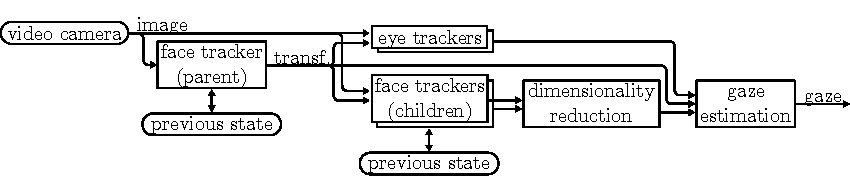
\includegraphics{img/impl-overview.pdf}
	\caption{Overall scheme of gaze tracking.}\label{i:impl-overview}
\end{figure}

The pipeline of computation is presented in Drawing \ref{i:impl-overview}.
Firstly, the face is locally tracked from the previous frame by the so-called parent tracker.
Only if this step fails, the program executes a global face localization procedure.
This first step results in a geometric image transformation.

Next, the precise position of both eyes is established within a reasonable region in the face.
This step requires the face to be localized properly in the image but since the eyes can move very quickly, no information from previous frames is taken into account.

Finally, the 6 degrees of freedom of the head and the 2 degrees of freedom of each eye are fed into a gaze estimator that outputs coordinates in screen reference frame.

\section{Face tracking}
\label{s:impl-face}

\textit{Input:} reference image $\f{R}$ and current image $\f{I}$.\\
\textit{Output:} geometric transformation $\f T: \R^2 \to \R^2$ such that $\int_{\vec p \in \R^2} |\f{R}(\vec p) - \f{I}(\f{T}(\vec p))|^2$ is minimal.\footnote{
Both of the images are considered zero outside their bounds.
}\\

The tracking is split into two parts: a \textit{parent tracker} that covers the whole face, and several \textit{child trackers} that capture more subtle degrees of freedom.
All of the trackers are deformable templates along the lines of \cite{bouguet01}.

The reference image $R$ is a single frame that is used during the whole course of operation.
Although this approach does not tolerate long term changes (such as when the user takes on their glasses), it makes our method robust against slow drift of the trackers.

Each of the trackers minimizes the energy function
$$\int_{\vec p} |\f{R}(\vec p) - \f{I}(\f{T}(\vec p))|^2,$$
where $T: \R^2 \to \R^2$ is a differentiable image transformation.
Note that we do use the color information---this seems to be quite rare in the literature.

Depending on the motion model expressed by the transformation $\f T$, we get different kinds of trackers that also differ by their degrees of freedom (DoF):
\begin{itemize}
\item
Similarity transformation: 4 DoF.
The transformation is parametrized by a displacement vector, scale and rotation angle.

\item
Affinity over a quadrangle: 6 DoF.
The transformation is parametrized by its $2 \times 3$ affinity matrix.

\item
Affinity over a triangle: 6 DoF.
This motion is advantageous over the previous one because its parameters exactly correspond to the DoF number of the transformation.
The parameters are exactly the vertices of a triangle that defines the tracker area.
This is important, as explained below.

\item
Homography. 8 DoF.
Again, the parameters of this motion model are exactly the four vertices that define the tracker area.
Homography encompasses all possible views of a planar object.

\end{itemize}
For performance reasons, a motion model must be chosen at compilation time, and it is shared by all the trackers.

We discretize the formula as a pixel-by-pixel sum and optimize it by gradient descent.
The derivatives of the transformation are computed analytically.
In case of the homography motion model, these derivatives are not quite obvious to formulate, and as such, they have been described in Section \ref{s:algo-dhomo}.
The formulas for calculating a triangle affinity are comparatively simple, but nevertheless, they have been summarized in Section \ref{s:algo-daff}.

In order to allow large-scale movement, all of the trackers operate upon an \textit{image pyramid}.
The pyramid is defined by downsampling the input image to half its resolution in a recursive manner.
The top level of the pyramid is an image too small to be downsampled.
The tracking starts by a quick estimate on the top level, and this information is successively refined until the bottom level with the original input resolution.

Assuming that the top level of the pyramid is correct, it is enough to refine the trackers up to the current pixel scale.
Any greater displacement should have been handled in the levels above.
Thanks to this assumption, only few steps of gradient descent (possibly just one) are necessary on each level of the pyramid.
That in turn allows us to track large displacements in real time.

The parent tracker provides a reference frame for all other features (e.g., eye trackers) and it supplies the most important parameters to gaze estimation.
In order to gain some robustness against changes in lighting, the parent tracker is color-normalized.

Our program supports two methods how the child trackers are managed.
These represent two major groups of tracking techniques in general: the feature-based and the appearance-based method.

\subsection{Markers}

This method relies on small-scale features that are usually present in the face and on skin---such as the eyebrows, nostrils, beard and skin defects.
Several small trackers are arbitrarily placed within the face area, each of them large just enough so as to track a single feature of the face.
Technically, it is possible to track any distinctive texture, so an automated feature detection such as the Harris corner detector (provided by a third-party library) performs well enough.

Each of the markers is allowed to freely move around.
(In contrast to the classical Deformable Parts Model such as in \cite{uricar12}, we do not calculate any penalty from their relative configuration.)
They are tracked from their previous known position relatively to the parent tracker.
If the tracking score of a marker drops below a certain limit or a marker escapes the face area, it is reset to its original position and tracking continues from there.

\subsection{Grid}

This method follows the approach of Active Appearance Models \cite{cootes01}.
The parent tracker is subdivided into a planar mesh, and each cell is responsible of tracking the corresponding part of the image.

In order for the cells to form a contiguous mesh, certain parameters of neighboring cells are bound together and need to be optimized concurrently.
Our implementation of the corresponding tracker methods does this explicitly since their parameters are the planar coordinates of their corner vertices.
During optimization, the derivatives are summed up in each grid vertex (nevertheless the number of cells that share it) and all grid vertices are updated at once.

This process is commonly done with a triangular mesh (i.e., barycentric cells), where the derivatives wrt. vertex coordinates are quite easy to derive.
Our extension of this method to a quadrangular mesh (i.e., homographic cells) relies on the concepts developed in sections \ref{s:algo-homo} and \ref{s:algo-dhomo}.

\section{Eye tracking}

\textit{Input:} iris radius $r \in \R$ and image $\f I$ centered at an expected eye location.\\
\textit{Output:} iris center $\vec c \in \R^2$.\\

\todo{further assumptions on the image necessary for good recognition}
\todo{list out the difficult factors and reference the table in Results}

Once the face itself has been tracked, the eyes can be easily located using their reference position.
The iris radius can also be extracted by multiplying the reference radius with a scale factor given by the face tracker.
Most of the face trackers induce non-uniform scaling, so it might seem appropriate that the eye shape will be an ellipse.
However, we assume that eyes are always directed towards the camera, so the limbus should retain a circular shape even if the face is stretched.

\todo{explain that we do not impose many constraints on the pupil occlusion, so the problem is actually very hard.}

There are a plenty of eye trackers available in our program.
From a broader perspective, we took four different approaches:
\begin{itemize}
\item Tracking the limbus. There should be a circle with a strong gradient directed outwards.
\item Tracking the iris. It should be radially symmetric with a strong gradient on the edges.
\item Segmentation. Skin, sclera, iris and pupil should each be uniform, but mutually different in color.
\item Machine learning. Instead of modeling, we can feed the image into a regression engine.
\end{itemize}

Acknowledging that the scale (e.g., the radius $r$) can be only a few pixels, we aim for a subpixel precision.
That is a meaningful pursuit thanks to the continuous image model defined in Section \ref{s.imagemodel}.

However, many of the algorithms to be presented are based on pixel by pixel evaluation of a scoring function.
In such cases, it is not very appropriate to evaluate at fractional coordinates.
Instead, we fit a quadratic polynomial to several score values around the maximal pixel, and output the maximum of this polynomial as the global maximum.

The following methods are available to the host application:

\subsection{Limbus gradient}
This method relies on the edge between the iris and the sclera.
Assuming that the iris is much darker than the sclera, their shared boundary (the limbus) should be sensed as a circle of high contrast.
Curve fitting to detected edge pixels can provide very precise results \cite{kassner14}.
Given the image resolution we work with, the usual approach based on a Canny filter and ellipse fitting is not viable.
Instead, we propose an iterative optimization scheme that will directly fit a circle to the image gradient.

We assume the eyelids be of uniform color, so they have zero value in the gradient domain and can be neglected.

\todo{formulate the energy function}
This function is minimized by gradient descent.
It is important to note that optimization of a function based on image gradient requires image derivatives of second order to be calculated.
\todo{if there is a citation for this:}
These are often considered unstable and avoided in the literature.
In our case, the function to be optimized appears to be smooth enough, and the algorithm converges well if initialized a few pixels from the correct solution.

This method is designed for refining an estimated eye position on the subpixel level, so it performs well when coupled with another eye tracking method.
If executed alone, it often fails to locate the global optimum.

\subsection{Hough Transformation}
We can use a voting scheme to find the limbus center, as described in Section \ref{s:algo-hough}.
\todo{used in \cite{leo14,zhang13}}

A free parameter is yet to define: the resolution of the voting grid.
Using each pixel as a voting bin is usually the best choice, but it may fail on blurry images of high resolution because the votes will be distributed quite randomly over a wide region around the true center.

\subsection{Dark iris correlation}

Assuming that the iris is a dark disc and the rest of the image is much brighter, we can use basic template matching techniques to locate it.
This technique is very popular \cite{zhu12,george16}
An appropriately fast and reliable one is the normalized correlation, using a slightly blurred black circle as the template.

\todo{formula for the kernel}

This method appears to work especially well when tested in regions where the majority of people are brown-eyed and with white skin.
It can also easily get confused by dark spots around the eyes, such as glass rims or strong makeup.
Finally, this method requires most of the iris to be visible, which need not be true because of the viewing angle and the user's personal habit.

\subsection{Personalized iris correlation}
The assumption of dark iris is wrong: the iris is often much brighter than the surrounding skin, especially in the case of blue-eyed people.
In fact, the iris image varies so greatly among individuals that it is often advocated as a means of identification or authentification \cite{bowyer16}.
We can, however, rely on the whole iris region (including the pupil) to be a constant, radially symmetric image, and locate it using a personalized template.
Acquiring this template requires the user to wide open their eyes, so that the whole limbus is visible.

For tracking a colored object, it is again reasonable to use the normalized correlation.

\subsection{Iris radial symmetry}

It may be considerably difficult to obtain a reliable iris image, and generally speaking it is a calibration step that we wish to avoid.
Instead, we can use the sole fact that the iris is a radially symmetric object on a white background.
An example of a filter based on radial symmetry can be found in \cite{leo14}.
Hereby we design a novel robust algorithm that exploit color information.

The iris colors are recalculated for each frame and each eye position, so only few free parameters remain.

This algorithm has built-in skin masking, so that whole segments of the iris are ignored where the limbus is not visible.

\todo{Add some intro -- let us define the following functions}
\begin{itemize}
\item
Angular limbus score $\f{limbus}(\alpha)$ is the gradient magnitude $|\nabla \f{I}(\vec p)|$ where $\arctan(\vec p) = \alpha$ and $|\vec p| = r$.

\item
Radial color $\f{mean}(t)$ is a mean value of the set $\{\f{I}(\vec p) \text{ for all } |\vec p| = t \}$.

\item
Angular iris score $\f{iris}(\alpha)$ is the weighted arithmetic mean of the set $\{\f{I}(\vec p)$ for all $\arctan(\vec p) = \alpha \}$.
The weight is $\f{w}(\vec p) = t \cdot (c - |\f{image}(\vec p) - \f{mean}(t)|)$, clamped to zero, with $t = |\vec p|$ and $c$ being a value appropriately chosen.

\end{itemize}
The total score is defined as $\int_\alpha \f{limbus}(\alpha) \cdot \f{iris}(\alpha)$.

Note that the formula for $\f{mean}(t)$ has not been specified yet.
Using the arithmetic mean may have a bad impact on the overall success rate.
It is appropriate here to use a more robust formula such as the median.

There are essentialy two ways how to generaze the median to color pixels.
Firstly, we can pick the median value as sorted by a scalar value (e.g., brightness).
This approach becomes unpredictable if many different colors have the same brightness, and specifically in the case of skin tones and iris color, this may be an issue.

The second option is to define the median of set $S$ as the value $\vec m \in S$ such that the sum of distances $\sum_{\vec x \in S} |\vec m - \vec x|$ is minimized.
This formula is consistent with the one-dimensional case and is valid in any metric space.
Unfortunately, efficient algorithms to compute this value are too sophisticated, so we loop over $S$ explicitly.

This function is computationally expensive and, depending on the method for mean color calculation, difficult to optimize locally.
Our program does not even contain the code to calculate the derivatives.
This tracker uses exhaustive search to find the global minimum within a crop-out image.

\subsection{Skin masking}

Skin, including the eyelids, can be detected quite easily by an analysis of its color.
This approach is perhaps too naive to be widely advocated in the literature, but it can be found in software libraries such as \cite{deepgaze}.

We allow each of the eye trackers presented so far to be coupled with a HSV (hue-saturation-value) detector tuned for skin tones.
Pixels whose HSV vector lies within a user-defined cube are excluded from eye fitting.

The mapping of RGB values to HSV is a piecewise linear function:
\todo{formula}

It is important to note the heuristic aspects of this approach.
\todo{HSV, sRGB, the cube -- lighting, skin color etc.}

Since there are usually many distractive features around the eyes, such as the eyelashes and makeup, the mask is pre-processed so as to have a smooth boundary and to cover nearby black splotches.

\todo{This is yet to be coded and tested.}

\subsection{Combined estimator}

Having implemented several algorithms for the same task, it is possible to adaptively combine their results.
An example of two different algorithms summing their results can be found in \cite{leo14}.
A more common approach is to run several trackers in sequence, such as in \cite{wang16,george16,zhu12}.
Our program supports can combine both of these options in a tree-like manner arbitrarily.

Choosing several trackers that are sensitive to different deteriorations of the image, we can trade off some computational time for much robustness and precision.
Each of the trackers chosen should obviously fail in different conditions so that a majority of them is correct on every image.
For an empiric comparison on reasonable selection of trackers for a combined estimator, see Section \ref{s:results-eyecovar}.

After letting each of the selected trackers cast a vote, it is possible to combine them robustly (as compared to the arithmetic average).
It is very much possible that one or more of the trackers fail.
We have very little prior information about the eye position, but we can exploit the distances among the votes.

In the case of three trackers running in parallel, we can heuristically throw out the vote that is significantly far away from the remaining two.
For a higher count of votes (assuming still that the number is reasonably small), this can be generalized as the subset with minimal expected variance.
In order to find it, we explicitly loop over all the subsets.
The average of this subset is the result of the combined estimator.

Note that in the case of two votes, their arithmetic mean is the only option.
In the three-vote case, either a mean of two or the mean of all three can be selected depending on their relative distances.

\begin{lemma}
Given a set $X = \{\vec x^i\}$ of samples from a normal distribution, the expected value of the variance $\var X$ is
$$\E\var (\vec x) = \frac 1 {n - 1} \sum_i (\vec x^i - \hatvec x),$$
where $\hatvec x$ is the arithmetic mean of $X$.
\end{lemma}
\begin{proof}
\todo{cite or derive}
\end{proof}

Another option is to run several algorithms in sequence.
In this setting, the first algorithm provides a rough estimate that is subsequently refined by the remaining ones.
Since most of our eye trackers use exhaustive pixel-by-pixel search, there are only few meaningful configurations of this kind.

\section{Gaze estimation}
\label{s:impl-gaze}

\textit{Input:} vectors $\vec e \in \R^n$ and $\vec f \in \R^m$ and \textit{gaze parameters} as defined below.\\
\textit{Output:} vector $\vec p \in \R^2$.\\

\begin{definition} \label{d:gaze-parameters}
The \textit{gaze parameters} consist of an orthonormal basis $\mat P \in \R^{2\times n}$ and a homography $\mat H \in \R^{3 \times (m+3)}$.
\end{definition}

Given the vector $\vec f$ obtained from face tracking and vector $\vec e$ obtained from eye tracking, and using the scene model described in Section \ref{s:gaze-model}, we wish to estimate the on-screen position $\vec p$ (in pixel units).
Commonly used approximation methods for this purpose vary greatly from simple approximations \cite{zhu12} more flexible ones \cite{kassner14,yucel09} and thorough geometric models \cite{villanueva08,wang16}.

Computer screen is a plane in space, with pixels aligned in a regular square grid.
If the face and the eyes were also planar objects, then the gaze in screen coordinates would be related to the face and eyes position by a projectivity.
This is obviously not the case, and the face transformation has many more degrees of freedom than a planar rigid body would.
 
In order to properly model the mapping from our face and eye parameter space to 2-dimensional gaze, we would have to actually approximate the three-dimensional model of the face.
Many programs have been published (e.g., \cite{fanelli11}) that follow this path.
In general, it requires some prior information about the shape of the face, and much tuning to calibrate a 3d model precisely enough.
To avoid these issues, we decided for a simpler approach.

We decided to actually assume the gaze is given by a projective transformation of the face and eye parameters.
This approach is limited and even in theory, it does never perfectly fit the data.
On the other hand, homographies have a solid mathematical background, and they can be estimated quickly and robustly from data.
All invertible homographies form a group that contains the group of invertible affine transformations, and they can also implicitly model inverse proportionalities among their parameters.


\todo{combine with the following section in a meaningful manner}

\section{Calibration}

\textit{Input:} interactive session with the user.\\
\textit{Output:} gaze parameters (see Definition \ref{d:gaze-parameters}).\\

The purpose of calibration is to learn all necessary parameters about the user's face and the geometry of the screen relatively to the camera.
Depending on the tracking quality, the time spent to measure all necessary information may vary.

During the calibration, roughly speaking, the user is asked to watch specific points on screen and their face and eyes are tracked.
For each screen position measured this way, the face tracker provides many parameters.
Some of these have an implicit meaning, others can be processed to extract useful information and yet others are just noise.
We fit a homography mapping some of the face parameters and the eye parameters to each known gaze position.

In the beginning of the calibration session, a single frame is acquired from the camera.
Depending on the application, either the program locates the user's face and eyes, or asks the user to do so manually.
For the automatic face and eye localization, a boosted random forest classifier is used within a sliding window.

The calibration session proceeds by presenting the user with a dot moving around the screen.
The user is asked to watch the dot carefully until it disappears.
In order to make the movement more predictable, the dot moves along a smooth curve with piecewise constant curvature, and a patch of this curve is being drawn ahead of time.
The calculated parameters from face tracking are recorded along with the current on-screen position of the dot.

It is meaningful to extract four basic parameters about a face tracker: its position within the image, its on-screen rotation and scale.
The head (as a rigid body) has two more parameters to be covered, but there is a virtually unlimited number of extra parameters that can be obtained from detailed tracking of the face.
Face pose is unknown in each frame, and possibly constant, so there is a high danger of overfitting.
We cut down the dimensionality by Principal Component Analysis: out of the extra parameters, only the two largest principal components are preserved.

It is possible that the user's gaze twitches for a moment, or that the gaze tracking fails in several frames.
In order to ignore these faulty measurements, we employ a Ransac fitting repetitively.
As soon as a fit collects a large enough support of measurements, the calibration procedure stops and outputs the homography it acquired.

